\documentclass[11pt]{article}
\usepackage{geometry}
\geometry{letterpaper, margin=1in}
\usepackage[utf8]{inputenc}
\usepackage{graphicx}
\usepackage{upgreek}
\usepackage{hyperref}
\usepackage[T1]{fontenc}
\usepackage{amsmath}
\usepackage[colorinlistoftodos]{todonotes}
\usepackage{float}
\usepackage{minted} 
\usepackage{scalerel}

\title{ECE532S Digital Systems Design \\ \vspace{0.4cm}
       \Large Tutorial 6 - Creating and Packaging a Custom IP \\ \vspace{0.4cm}
       \small Last Updated: July, 2019}
\author{ }
\date{ }

\begin{document}
\maketitle
\vspace{-1cm}

In previous tutorials we've used IP cores provided by Xilinx to implement various functionalities. In this tutorial, we'll go through the project flow for creating your own IP cores. In particular, we will be creating an IP core that uses an AXI interface, such that our core can be controlled by a MicroBlaze system.




\section{Creating the AXI IP}
\label{sec:create_axi_ip}
Launch Vivado and select \textbf{Manage IP... $\rightarrow$ New IP Location} under the \textit{Tasks} section of the Vivado Launch screen. Press \textbf{Next} and then select the part number that corresponds with the FPGA on the Nexsys FPGA, the \textbf{xc7a100tcsg324-1}. In the \textit{IP Location} field, select the folder to create a new IP repository. From the window toolbar, select \textbf{Tools $\rightarrow$ Create and Package IP...}, which will bring up the \textit{Create New IP Wizard}. Press \textbf{Next} and then select the \textbf{Create a new AXI4 peripheral} option, as shown in Figure~\ref{fig:create_axi_ip}. Press \textbf{Next}.

\begin{figure}[!h]
    \centering
    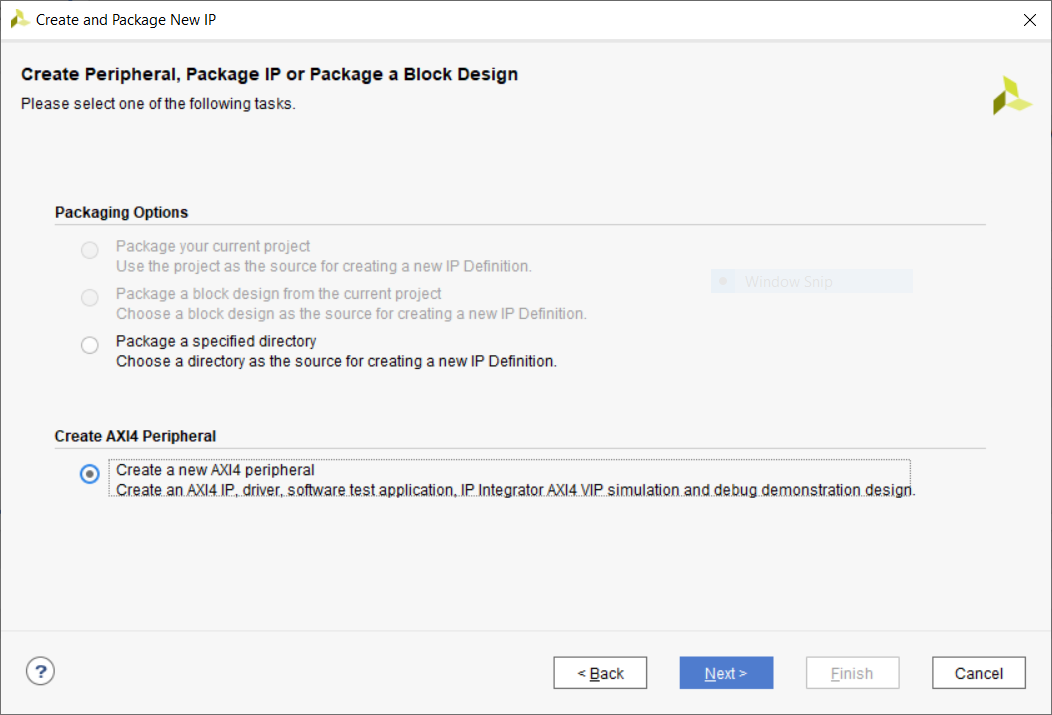
\includegraphics[width=0.9\textwidth]{images/create_axi_ip.png}
    \caption{Create new IP Wizard, selecting AXI4 peripheral}
    \label{fig:create_axi_ip}
\end{figure}

In the next window, we can select a name and version number for our new IP, we'll leave these settings at the default value. The \textit{IP Location} field determines where the newly created IP will be stored, and by default it's location will be within a subfolder titled \textit{ip\_repo} in the directory selected at the beginning of this section. Click \textbf{Next} to select the parameters of the new AXI IP. This \textit{AXI Interfaces} pane, shown in Figure~\ref{fig:create_axi_ip_options}, allows you to choose which and the number of AXI interfaces to include in the AXI IP. The middle section of this window lists all of the interfaces currently added, and allows for more interfaces to be added. The right section of this window shows the configuration for the selected AXI Interfaces. 

\begin{figure}[!h]
    \centering
    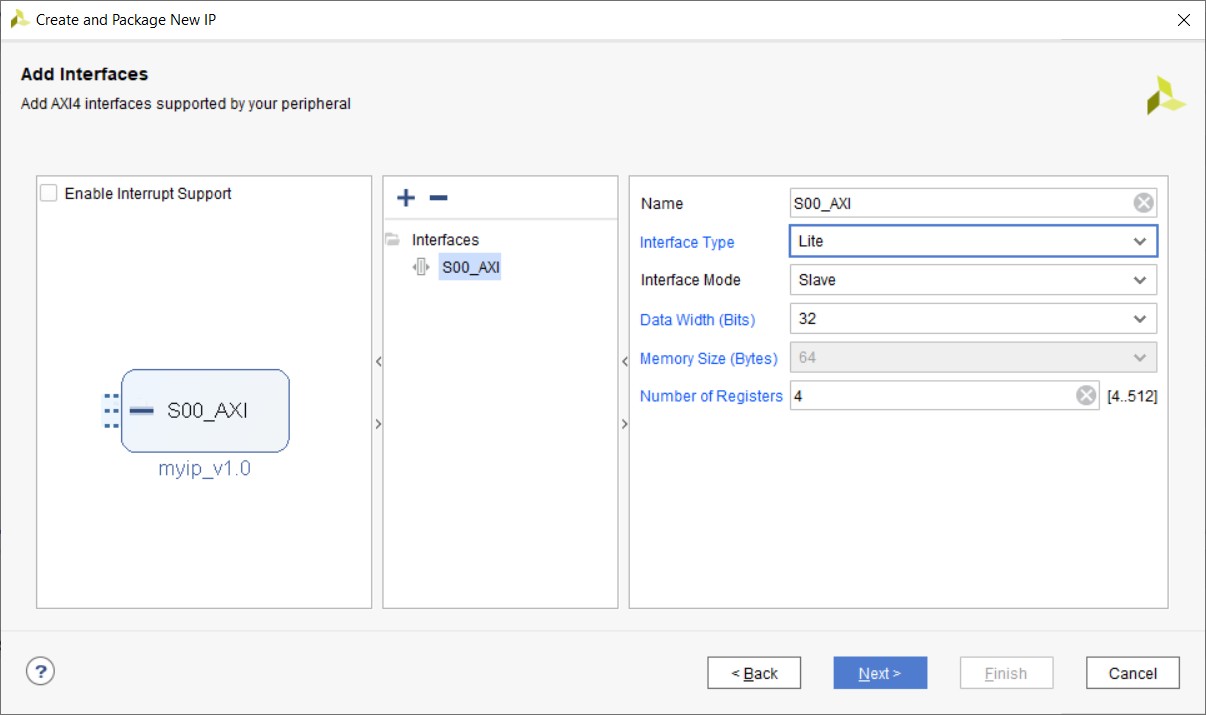
\includegraphics[width=0.9\textwidth]{images/create_axi_ip_options.png}
    \caption{Create new IP Wizard, AXI interfaces selection}
    \label{fig:create_axi_ip_options}
\end{figure}

The first option of note is the \textit{Interface Type} field. The AXI4 standard defines 3 main types of interfaces, the AXI4-full, the AXI4-lite, and the AXI-Stream. AXI4-full and AXI4-Lite are both memory mapped interfaces that can be accessed directly from a MicroBlaze. The AXI4-full interface supports burst accesses, and as such is generally used for high bandwidth interfaces. The AXI4-lite interface is simpler and generally used for peripherals that have a small number of registers to be accessed from the MicroBlaze. The AXI-Stream interface is generally used to encapsulate streaming data, such as network streams of video streams. For the purposes of this tutorial, we'll be creating an AXI-lite interface, so select \textbf{Lite} for the \textit{Interface Type}, select \textbf{Slave} for the \textit{Interface Mode} (i.e. the IP core is read/written to, rather than initiating reads and writes itself), and set the \textit{Number of Registers} to \textbf{4}. Press \textbf{Next} and then select \textbf{Edit IP} under \textit{Next Steps} and press \textbf{Finish}. 

This will open a new Vivado project for the IP. Under sources you will see both the Verilog source and a component.xml that describes your IP in IP-XACT format that the IP Integrator can understand. There are two sources, a top level \textit{myip\_v1\_0.v} and an interface module \textit{my\_ip\_v1\_0\_S00\_AXI}. For this design the top-level module just wraps the \textit{my\_ip\_v1\_0\_S00\_AXI} module (see Figure~\ref{fig:ip_hier}).

\begin{figure}[!h]
    \centering
    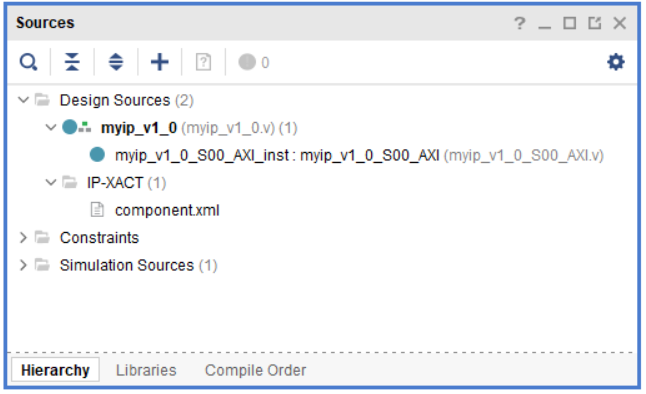
\includegraphics[width=0.7\textwidth]{images/ip_hier.png}
    \caption{AXI IP file hierarchy}
    \label{fig:ip_hier}
\end{figure}




\section{Understanding the AXI Lite Protocol}
\label{sec:understand_axi}
The template core implements a simple AXI lite slave interface and here we will describe a few basics of the AXI interface. The AXI protocol consists of five channels (the Verilog signals are prefixed with the parenthesized characters): 

\begin{itemize}
    \item Read Address (AR)
    \item Read Data (R)
    \item Write Address (AW)
    \item Write Data (W)
    \item Write Response (B)
\end{itemize}

\noindent
In general all channels communicate using READY/VALID handshaking. Only when the
sender asserts and valid signal and the receiver asserts a ready signal can data flow.


\subsection{Write Operations}
Write operations use the write address, write data and write response channels. Since this core is a slave, the address and data are inputs given by the master telling the slave where and what to write. The response channel is an output for acknowledging the transfer. Look for the assignment of the AWREADY, WREADY and AWADDR (write address data) signals. This implementation sets the ready signals high and gets the address when both address and data channels are valid. In the next cycle, the data to be written (WDATA) is stored in the addressed slave
register and BVALID is asserted.

\subsection{Read Operations}
Read operations only use an address and data channel. Like the write channel, the address is registered one cycle before the data is transferred. However, in this case the data is an output from our slave containing the value of the addressed register. The logic for read operations is below the write
operations in the template Verilog implementation. You are encouraged to examine the code more closely to more fully understand the functionality.




\section{Modifying the AXI IP}
\label{sec:mod_axi_ip}
The skeleton Verilog code handles reading and writing the four slave registers. We will now insert an adder to produce a sum output of our four slave registers. There are two main areas that we generally modify within this skeleton code, and each is annotated as such with comments. First, the section that appears as follows:

\begin{minted}
[
framesep=2mm,
baselinestretch=1.2,
bgcolor=white,
breaklines,
]
{verilog}
    // Users to add ports here

    // User ports ends
    // Do not modify the ports beyond this line
\end{minted}

\noindent
We want to add a single output port that caries the sum of all of our registers within our AXI-Lite IP. Modify this section of code to appear as follows:

\begin{minted}
[
framesep=2mm,
baselinestretch=1.2,
bgcolor=white,
breaklines,
]
{verilog}
    // Users to add ports here
    output [7:0] sum,
    // User ports ends
    // Do not modify the ports beyond this line
\end{minted}

\noindent
In future custom IP designs, you could add any number of signals here that you would like to appear on the interface of the IP core. The next section of that we can modify appears as follows later in the code:

\begin{minted}
[
framesep=2mm,
baselinestretch=1.2,
bgcolor=white,
breaklines,
]
{verilog}
    // Add user logic here

    // User logic ends
\end{minted}

\noindent
We will add logic here that determines the sum from our register values. Modify this section of code to appear as follows:

\begin{minted}
[
framesep=2mm,
baselinestretch=1.2,
bgcolor=white,
breaklines,
]
{verilog}
    // Add user logic here
    assign sum = slv_reg0[7:0] + slv_reg1[7:0] + slv_reg2[7:0] + slv_reg3[7:0];   
    // User logic ends
\end{minted}

\noindent
Now that we have the port added and the logic to implement our required functionality, we need to modify the wrapper verilog file to carry this signal to the top level of our design. The top level file, titled \textit{myip\_v1\_0.v}, also contains an area to add ports:

\newpage
\begin{minted}
[
framesep=2mm,
baselinestretch=1.2,
bgcolor=white,
breaklines,
]
{verilog}
    // Users to add ports here

    // User ports ends
    // Do not modify the ports beyond this line
\end{minted}

\noindent
Modify it to add a sum port just as we did with the \textit{S00\_AXI} module. Next, we have to connect this signal in the top level wrapper to the instance of the \textit{S00\_AXI} module. CHange the instantiation of the inner module such that it appears as follows:

\begin{minted}
[
framesep=2mm,
baselinestretch=1.2,
bgcolor=white,
breaklines,
]
{verilog}
    myip_v1_0_S00_AXI # ( 
        .C_S_AXI_DATA_WIDTH(C_S00_AXI_DATA_WIDTH),
        .C_S_AXI_ADDR_WIDTH(C_S00_AXI_ADDR_WIDTH)
    ) myip_v1_0_S00_AXI_inst (
        .sum(sum), // We added this connection
        .S_AXI_ACLK(s00_axi_aclk),
        .S_AXI_ARESETN(s00_axi_aresetn),
        .S_AXI_AWADDR(s00_axi_awaddr),
        .S_AXI_AWPROT(s00_axi_awprot),
        .S_AXI_AWVALID(s00_axi_awvalid),
        .S_AXI_AWREADY(s00_axi_awready),
        .S_AXI_WDATA(s00_axi_wdata),
        .S_AXI_WSTRB(s00_axi_wstrb),
        .S_AXI_WVALID(s00_axi_wvalid),
        .S_AXI_WREADY(s00_axi_wready),
        .S_AXI_BRESP(s00_axi_bresp),
        .S_AXI_BVALID(s00_axi_bvalid),
        .S_AXI_BREADY(s00_axi_bready),
        .S_AXI_ARADDR(s00_axi_araddr),
        .S_AXI_ARPROT(s00_axi_arprot),
        .S_AXI_ARVALID(s00_axi_arvalid),
        .S_AXI_ARREADY(s00_axi_arready),
        .S_AXI_RDATA(s00_axi_rdata),
        .S_AXI_RRESP(s00_axi_rresp),
        .S_AXI_RVALID(s00_axi_rvalid),
        .S_AXI_RREADY(s00_axi_rready)
    );
\end{minted}

\noindent
Note that the only modification we've made is that we've added the connection to the \textit{sum} port. Now that we've implemented the functionality of our custom core within the skeleton code, we can proceed to package our IP. \textbf{Save} all your sources and open the \textit{Package IP} tab. When we started creating this IP, all of the steps in the \textit{Package IP} tab displayed a 
\scalerel*{
\includegraphics{images/ip_pack_check.png}}{(}
icon to indicate that the step is complete. Now that we've changed some of the source files, a
\scalerel*{
\includegraphics{images/ip_pack_change.png}}{(}
icon indicates that the step needs to be updated based on the changes. Open the first packaging step that needs to be updated (it should be \textit{File Groups}, and you should notice a \textit{Merge changes from File Groups Wizard} prompt, as in Figure~\ref{fig:merge_changes}. Click \textbf{Merge changes from File Groups Wizard} and the step should transition to complete. Repeat this for each of the \textit{Packaging Steps}. Note, the \textit{Merge changes} wizard may complete multiple steps at a times.

\begin{figure}[!h]
    \centering
    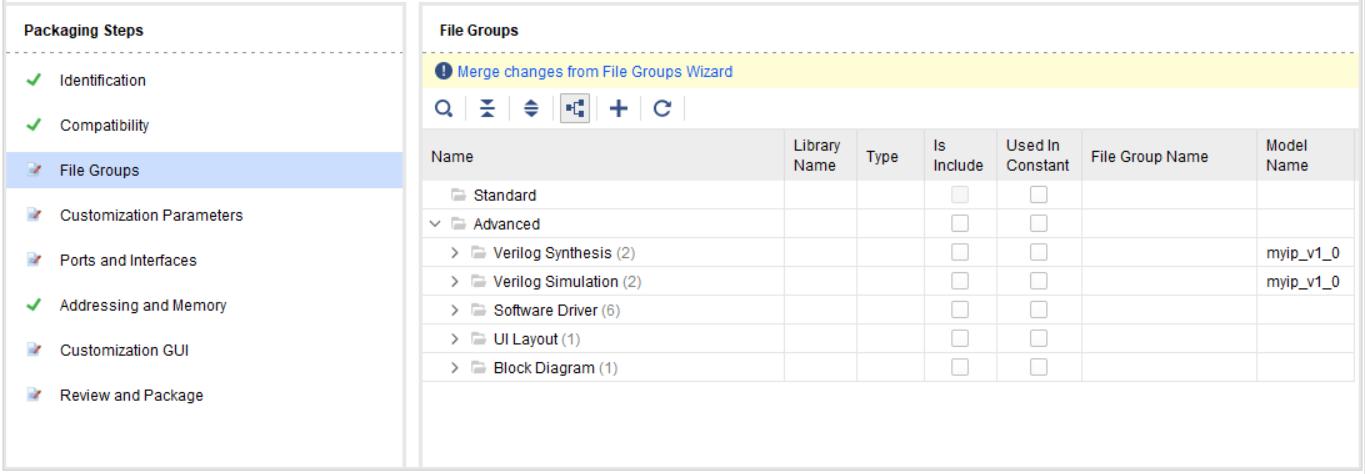
\includegraphics[width=0.95\textwidth]{images/merge_changes.png}
    \caption{IP packaging steps, with merge changes wizard prompt}
    \label{fig:merge_changes}
\end{figure}

While we don't need to make any changes from the defaults selected by the wizard, it is still important to know what the purpose of each of these \textit{Packaging Steps} is. The \textit{Identification} step allow you to enter the name, version, and description for your core. Here you will generally update the version with every update. The \textit{Compatibility} step allows you to select what FPGAs the IP is compatible with; you'll only need to modify this if your Verilog includes modules that in themselves are not compatible with all Xilinx FPGAs (usually these are devices primitives). The \textit{File Groups} step lists all of the files included in the IP, and is where you would select to add any newly created verilog files to the IP. The \textit{Customization Parameters} lists all of the Verilog parameters within your top level module; you can change settings for them here. The \textit{Ports and Interfaces} should list all of the top level ports of your design; check to make sure the \textit{sum} port was added as an output. The \textit{Addressing and Memory} step lists all memory regions of your IP Core. The \textit{Customization GUI} step allows you to change what the GUI looks like for configuring your core. Finally, select the \textbf{Review and Package} step to finish the packaging process. Press \textbf{Re-Package IP} to package the IP with all of the changes we made. You can now close the IP project.




\section{Using the Custom IP}
\label{sec:using_ip}
Open or recreate the project from tutorial~3 (create a copy of the project directory if you want to preserve the version of the project for reference later). Open the settings window from \textbf{Tools $\rightarrow$ Settings...} and expand the \textit{IP} heading in the left pane. Select \textbf{Repository} to bring up the \textit{IP Repository} settings in the right pane. Press the 
\scalerel*{
\includegraphics{images/add_repo.png}}{(}
button to add a new IP repository to the project. Navigate to the \textit{ip\_repo} subfolder of the directory you selected in the first step of this tutorial, and press \textbf{Select}. The window that comes up lists all IP found in that repository; you should see the new custom IP we created listed. See Figure~\ref{fig:ip_repo_added} for reference.

\begin{figure}[!h]
    \centering
    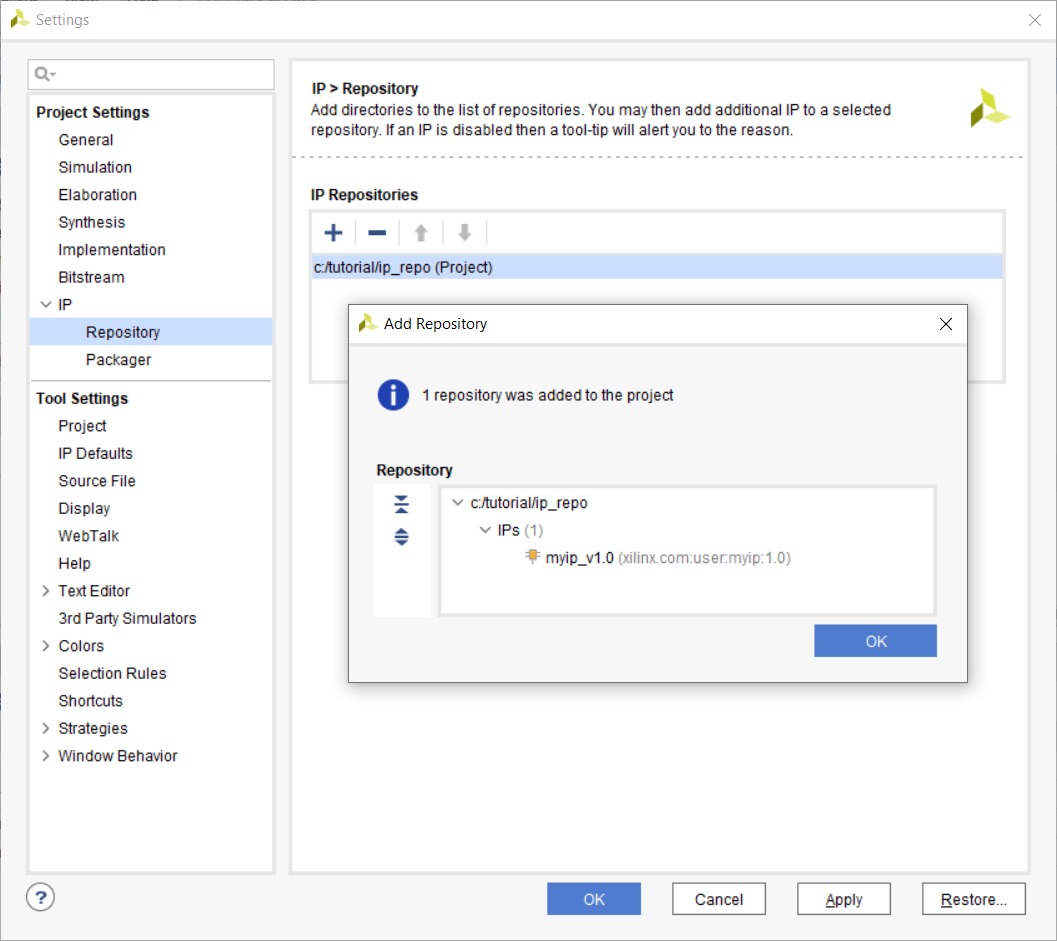
\includegraphics[width=0.9\textwidth]{images/ip_repo_added.png}
    \caption{IPs listed after adding an IP repository}
    \label{fig:ip_repo_added}
\end{figure}

Open the block diagram in your project. In order to simplify the project, go ahead and \textbf{delete} the \textit{MIG}, as well as the \textit{Processor System Reset} connected to the \textit{MIG}. If your project had an \textit{ILA} that was connected to the \textit{MIG}, you can \textbf{delete} that core as well. Now \textbf{right click} anywhere in the block diagram window and select \textbf{Add IP...}. Search for the IP core we just created, titled \textit{myip\_v1.0}, and add it to your project. Click \textbf{Run Connection Automation} in order to automatically connect the AXI signal on our custom IP Core to the AXI interconnect. \textbf{Right click} anywhere in the editor window and select \textbf{Create Port}. Make a port called led, set as \textbf{Output}, as a vector of size 7 down to 0. Connect this newly created port to the sum port of our core. You should now have an IP core in the project connected as per Figure~\ref{fig:block_w_core}. 

\begin{figure}[!h]
    \centering
    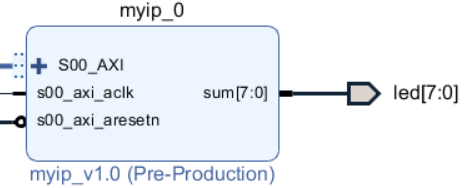
\includegraphics[width=0.6\textwidth]{images/block_w_core.png}
    \caption{The custom IP core connected within IP Integrator}
    \label{fig:block_w_core}
\end{figure}

We need to add a constraint file to our project to connect this new output value to the leds. Close the block diagram view. \textbf{Right click} the block diagram in the source window and select \textbf{Create HDL Wrapper} to regenerate the block diagram wrapper. Open the verilog wrapper and verify that the \textit{led} signal has been added as an output of the top level module. Note, we usually check the wrapper since the name of the signal in the wrapper doesn't always exactly match the name we gave to the signal in the block diagram view. Add a new constraint file to the project with the contents of Figure~\ref{fig:xdc_file}.

\begin{figure}[!h]
\centering
\begin{minted}
[
frame=lines,
framesep=2mm,
baselinestretch=1.2,
bgcolor=white,
fontsize=\footnotesize,
linenos,
breaklines,
]
{tcl}
set_property PACKAGE_PIN H17 [get_ports led[0]]
set_property IOSTANDARD LVCMOS33 [get_ports led[0]]
set_property PACKAGE_PIN K15 [get_ports led[1]]
set_property IOSTANDARD LVCMOS33 [get_ports led[1]]
set_property PACKAGE_PIN J13 [get_ports led[2]]
set_property IOSTANDARD LVCMOS33 [get_ports led[2]]
set_property PACKAGE_PIN N14 [get_ports led[3]]
set_property IOSTANDARD LVCMOS33 [get_ports led[3]]
set_property PACKAGE_PIN R18 [get_ports led[4]]
set_property IOSTANDARD LVCMOS33 [get_ports led[4]]
set_property PACKAGE_PIN V17 [get_ports led[5]]
set_property IOSTANDARD LVCMOS33 [get_ports led[5]]
set_property PACKAGE_PIN U17 [get_ports led[6]]
set_property IOSTANDARD LVCMOS33 [get_ports led[6]]
set_property PACKAGE_PIN U16 [get_ports led[7]]
set_property IOSTANDARD LVCMOS33 [get_ports led[7]]
\end{minted}
\vspace{-0.7cm}
\caption{Contents of an XDC file to set pin constraints for the LEDs}
\label{fig:xdc_file}
\end{figure}

Run \textbf{Synthesis}, \textbf{Implementation}, \textbf{Generate Bitstream}, and \textbf{Export Hardware}, and then launch \textbf{Vivado SDK}. Open the \textit{helloworld} application and modify the contents of \textit{helloworld.c} to the contents of Figure~\ref{fig:app_custom_ip}. This is a very simple application that just writes random values to the different registers of our core. The output value produced will be the sum of these values, which is 87, or 01010111. Before running our project, remember to open one of the board support package include files, such as \textit{xi\_printf.h}, and press \textbf{F5} to refresh them (as we did in tutorial~4). Open the \textit{Run Configurations} windows and ensure the \textbf{Program FPGA} check box is checked and press \textbf{Apply} (we unchecked it in tutorial~4). Now press \textbf{Run} to run the application on the FPGA. Verify the functionality is as expected on the leds.

\begin{figure}[!h]
\centering
\begin{minted}
[
frame=lines,
framesep=2mm,
baselinestretch=1.2,
bgcolor=white,
fontsize=\footnotesize,
linenos,
breaklines,
]
{c}
#include <stdio.h>
#include "platform.h"
#include "xil_printf.h"
#include "xparameters.h"

volatile unsigned int* myip_base = (unsigned int*) XPAR_MYIP_0_S00_AXI_BASEADDR;

int main()
{
    init_platform();

    print("Writing to Registers\n\r");
    *(myip_base+0) = 7;
    *(myip_base+1) = 12;
    *(myip_base+2) = 67;
    *(myip_base+3) = 1;

    cleanup_platform();
    return 0;
}
\end{minted}
\vspace{-0.7cm}
\caption{Modified Hello World application using custom IP core}
\label{fig:app_custom_ip}
\end{figure}

When we created and packaged the custom IP, Xilinx also packaged a simple \textit{low level driver} for the IP. Open the \textit{myip.h} file in the \textit{include} folder of the board support package. Examine the contents to see how to use the driver. Now modify the \textit{helloworld.c} file to use the \textit{low level driver}, as shown in Figure~\ref{fig:app_custom_ip2}. Run this modified application and verify that we get the same expected output.

\begin{figure}[!h]
\centering
\begin{minted}
[
frame=lines,
framesep=2mm,
baselinestretch=1.2,
bgcolor=white,
fontsize=\footnotesize,
linenos,
breaklines,
]
{c}
#include <stdio.h>
#include "platform.h"
#include "xil_printf.h"
#include "xparameters.h"
#include "xil_io.h"
#include "myip.h"

int main()
{
	init_platform();

	print("Writing to Registers\n\r");
	MYIP_mWriteReg(XPAR_MYIP_0_S00_AXI_BASEADDR, MYIP_S00_AXI_SLV_REG0_OFFSET, 7);
	MYIP_mWriteReg(XPAR_MYIP_0_S00_AXI_BASEADDR, MYIP_S00_AXI_SLV_REG1_OFFSET, 12);
	MYIP_mWriteReg(XPAR_MYIP_0_S00_AXI_BASEADDR, MYIP_S00_AXI_SLV_REG2_OFFSET, 67);
	MYIP_mWriteReg(XPAR_MYIP_0_S00_AXI_BASEADDR, MYIP_S00_AXI_SLV_REG3_OFFSET, 1);

	cleanup_platform();
	return 0;
}
\end{minted}
\vspace{-0.7cm}
\caption{Modified Hello World application using custom IP core, with low-level driver}
\label{fig:app_custom_ip2}
\end{figure}




\section{Simulating the System}
\label{sec:sys_sim}
We need to be able to simulate our new AXI IP in order to effectively debug it. AXI interfaces can be difficult to simulate since the AXI protocol contains a number of signals, all of which must be varied together to create the proper read and write transactions. There are two ways to ease this simulation: using specially built simulation cores, and simulating the MicroBlaze system as a whole. An AXI simulation core will be covered in a future tutorial, here we will simulate the entire MicroBlaze system we just generated. Note, simulating the entire MicroBlaze system is a crude way to run a simulation for our AXI core, since this introduces the overhead of simulation the MicroBlaze processor, but it is a quick way to create a simulation that's easy to understand. In general, we prefer the simulation methods using simulation cores presented in the later tutorials.

\textbf{Close} the Vivado SDK and return to the Vivado project window. To simulate our MicroBlaze with the application we just wrote in \textit{Vivado SDK}, we need to associate the ELF file (the compiled executable) with the simulation sources. Open \textbf{Tools $\rightarrow$ Associate Elf Files...} to bring up the \textit{Associate ELF Files} window. Under \textit{simulation sources}, press the
\scalerel*{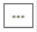
\includegraphics{images/browse_elf.png}}{(}
button beside the \textit{microblaze} component. In the new window click \textbf{Add Files...} and browse to your SDK folder. The SDK folder should be located within your Vivado project folder, with a name generally appended with with \textit{.sdk}. The ELF file should be located at a path similar to:

\begin{verbatim}
    <project name>.sdk/<application>/Debug/<application>.elf
\end{verbatim}

\noindent
where <application> is the name of the \textit{hellowworld} application you created in the \textit{Vivado SDK}. \textbf{Select} the ELF file and press \textbf{OK}. Make sure the newly added ELF file is highlighted and press \textbf{OK} again. You should now see the new elf file associated with the microblaze under simulation sources, as in Figure~\ref{fig:assoc_elf}. Press \textbf{OK}.

\begin{figure}[!h]
    \centering
    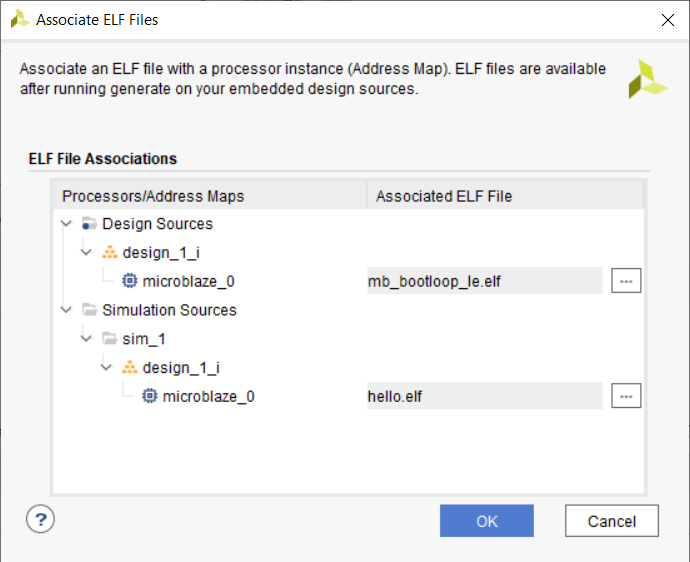
\includegraphics[width=0.7\textwidth]{images/assoc_elf.png}
    \caption{ELF file associated with the simulation microblaze}
    \label{fig:assoc_elf}
\end{figure}

Now we simply need to create a testbench that can drive the inputs of our top level module, the block diagram wrapper. Create a new simulation source with the contents of Figure~\ref{fig:system_tb}. Make sure the instantiation of the HDL wrapper matches the one from your project. This testbench simply connects wires to each of the top level ports of the HDL wrapper, and create a valid reset and clock signal. The reset signals is asserted for the first 40ns and the clock pulses with a period of 4ns. Note, we hardwired the \textit{usb\_uart\_rxd} to zero as we don't need to test the uart signals and we cannot leave an input signals unconnected.

\begin{figure}[!h]
\centering
\begin{minted}
[
frame=lines,
framesep=2mm,
baselinestretch=1.2,
bgcolor=white,
fontsize=\footnotesize,
linenos,
breaklines,
]
{verilog}
`timescale 1ns / 1ps

module tb();

    //Wires to connect to DUT
    reg clock, reset;
    wire usb_uart_rxd, usb_uart_txd;
    wire [7:0] led;

    //DUT
    design_1_wrapper dut(
        .sys_clock(clock),
        .reset(reset),
        .usb_uart_rxd(usb_uart_rxd),
        .usb_uart_txd(usb_uart_txd),
        .led(led)
    );
    
    assign usb_uart_rxd = 0;
    
    //Reset signal
    initial begin
        reset = 0;
        #40 reset = 1;
    end
    
    //Clock signal
    initial clock = 0;
    always begin
        #2 clock = ~clock;
    end

endmodule
\end{minted}
\vspace{-0.7cm}
\caption{Testbench to simulate the system}
\label{fig:system_tb}
\end{figure}

Run the behavioural simulation, select \textbf{Run Simulation $\rightarrow$ Run Behavioural Simulation} from the \textit{Simulation} heading in the \textit{FLow Navigator}. Once the behavioural simulation window opens, it will have simulated the design for some default amount of time (likely 500ns). This amount of time is not nearly enough time for the MicroBlaze to do some useful work, so we will have to run the simulation for a longer time. In any case, we want to add some signals from our custom IP first before proceeding. In the \textit{Scope} tab, expand the hierarchy until you find the lowest level module of the \textit{myip} core. Now, in the \textit{Objects} tab, find the four slave registers and drag them to your waveform window. See Figure~\ref{fig:ip_signals} for reference. Also add the \textit{sum} signals from the \textit{Objects} tab to the waveform viewer.

\begin{figure}[!h]
    \centering
    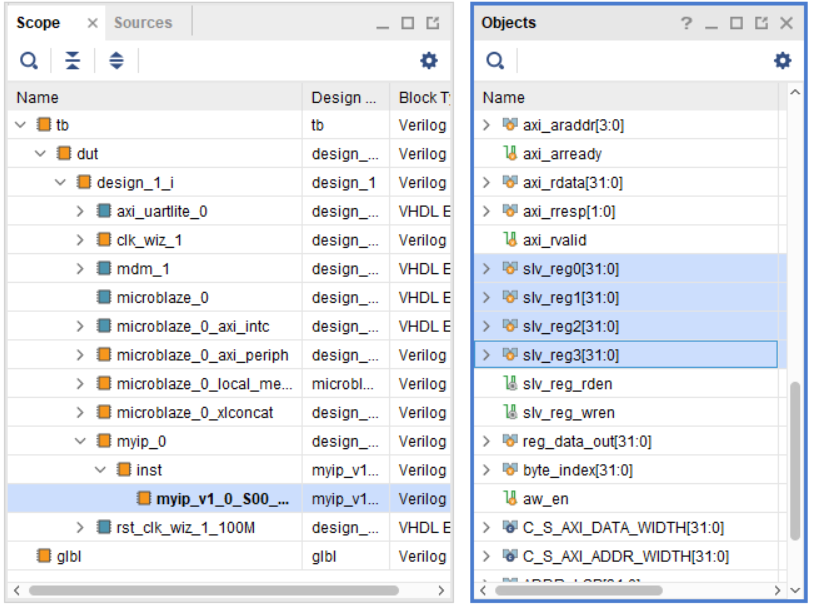
\includegraphics[width=0.8\textwidth]{images/ip_signals.png}
    \caption{The register signals within the AXI core}
    \label{fig:ip_signals}
\end{figure}

Once you've added the signals to the waveform viewer, proceed to run the simulation for 3 ms (note, milliseconds, not nanoseconds, use the drop down menu to select ms). Here you will notice the major downside of performing full system simulation, the simulation time can be incredibly long. This simulation may take up to a couple minutes to complete, but yet more complex systems or applications could take even longer to complete the simulation. This is because the processor is simulated at the RTL level. Once the simulation is complete, you should see an output like Figure~\ref{fig:sys_waveform}. Note, the radix for the registers and sum signal is set to \textit{Unsigned Decimal} in the figure.

\begin{figure}[!h]
    \centering
    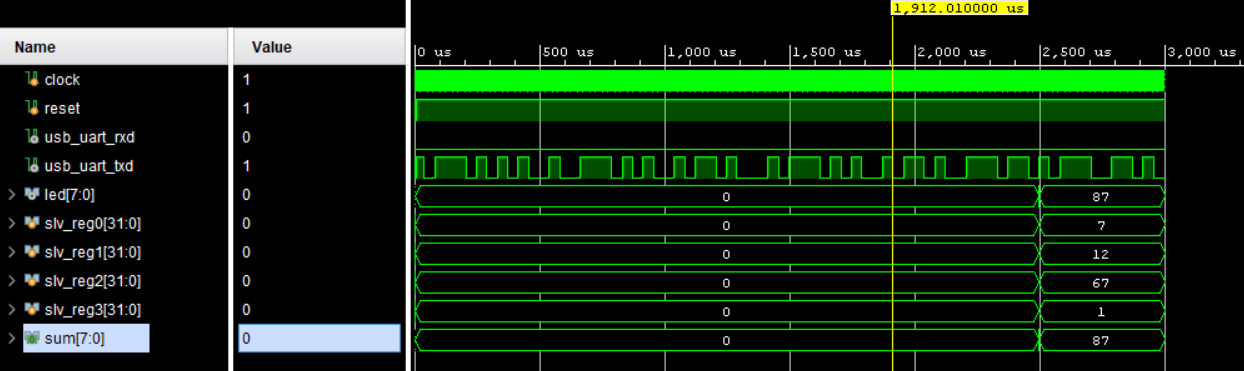
\includegraphics[width=\textwidth]{images/sys_waveform.png}
    \caption{Simulation waveform of the system simulation}
    \label{fig:sys_waveform}
\end{figure}

We notice that the write to our AXI registers are not made until around the 2.5ms point, which is over 600,000 cycles of the clock. In the meantime, the system seems to be trying to transmit something over the UART signal, likely the print statement from the application. Zoom in on the section where the register values are written to, you should now notice the gap between the successive write. This larger gap is because AXI-Lite doesn't support burst transfers, and as such each individual transfer takes longer to initiate. Here we also note that the sum value changes with each write to a register, which is something we wouldn't be able to see on the LEDs when testing on the physical board.




\section{Summary}
\label{sec:conc}
The Vivado flow for creating a custom IP allows us to wrap our own HDL cores such that they can included in Vivado projects through the block diagram editor. This flow even creates skeleton code with all of the functionality for any of the AXI protocols you'd like to include implemented for you. Note, the IP packaging flow demonstrated in this lab created a cor with AXI interfaces and corresponding generated skeleton code, though the IP packager can even be used with cores that have no AXI functionality. The IP core we created was instantiated in the block diagram from a previous tutorial, and we interfaced with it through a MicroBlaze program and system simulation.




\end{document}
